% This is "sig-alternate.tex" V2.1 April 2013
% This file should be compiled with V2.5 of "sig-alternate.cls" May 2012
%
% This example file demonstrates the use of the 'sig-alternate.cls'
% V2.5 LaTeX2e document class file. It is for those submitting
% articles to ACM Conference Proceedings WHO DO NOT WISH TO
% STRICTLY ADHERE TO THE SIGS (PUBS-BOARD-ENDORSED) STYLE.
% The 'sig-alternate.cls' file will produce a similar-looking,
% albeit, 'tighter' paper resulting in, invariably, fewer pages.
%
% ----------------------------------------------------------------------------------------------------------------
% This .tex file (and associated .cls V2.5) produces:
%       1) The Permission Statement
%       2) The Conference (location) Info information
%       3) The Copyright Line with ACM data
%       4) NO page numbers
%
% as against the acm_proc_article-sp.cls file which
% DOES NOT produce 1) thru' 3) above.
%
% Using 'sig-alternate.cls' you have control, however, from within
% the source .tex file, over both the CopyrightYear
% (defaulted to 200X) and the ACM Copyright Data
% (defaulted to X-XXXXX-XX-X/XX/XX).
% e.g.
% \CopyrightYear{2007} will cause 2007 to appear in the copyright line.
% \crdata{0-12345-67-8/90/12} will cause 0-12345-67-8/90/12 to appear in the copyright line.
%
% ---------------------------------------------------------------------------------------------------------------
% This .tex source is an example which *does* use
% the .bib file (from which the .bbl file % is produced).
% REMEMBER HOWEVER: After having produced the .bbl file,
% and prior to final submission, you *NEED* to 'insert'
% your .bbl file into your source .tex file so as to provide
% ONE 'self-contained' source file.
%
% ================= IF YOU HAVE QUESTIONS =======================
% Questions regarding the SIGS styles, SIGS policies and
% procedures, Conferences etc. should be sent to
% Adrienne Griscti (griscti@acm.org)
%
% Technical questions _only_ to
% Gerald Murray (murray@hq.acm.org)
% ===============================================================
%
% For tracking purposes - this is V2.0 - May 2012

\documentclass{sig-alternate-05-2015}
\usepackage{url}
\usepackage{epsfig}
\usepackage{makeidx}         % allows index generation
\usepackage{graphicx}        % standard LaTeX graphics tool
                             % when including figure files
\usepackage{multicol}        % used for the two-column index
\usepackage[bottom]{footmisc}% places footnotes at page bottom
\usepackage{float}           % H para posicionar figuras
\usepackage{booktabs}
\begin{document}

% Copyright
\setcopyright{acmcopyright}
%\setcopyright{acmlicensed}
%\setcopyright{rightsretained}
%\setcopyright{usgov}
%\setcopyright{usgovmixed}
%\setcopyright{cagov}
%\setcopyright{cagovmixed}


% DOI
\doi{10.475/123_4}

% ISBN
\isbn{123-4567-24-567/08/06}

%Conference
\conferenceinfo{MSR '16}{May 14-15, 2016, Austin, Texas, USA}

\acmPrice{\$15.00}

%
% --- Author Metadata here ---
\conferenceinfo{MSR}{'16 Austin, Texas USA}
%\CopyrightYear{2007} % Allows default copyright year (20XX) to be over-ridden - IF NEED BE.
%\crdata{0-12345-67-8/90/01}  % Allows default copyright data (0-89791-88-6/97/05) to be over-ridden - IF NEED BE.
% --- End of Author Metadata ---

\title{Who introduced the bug? The importance of the previous commit}
%\subtitle{[Extended Abstract]
%\titlenote{A full version of this paper is available as
%\textit{Author's Guide to Preparing ACM SIG Proceedings Using
%\LaTeX$2_\epsilon$\ and BibTeX} at
%\texttt{www.acm.org/eaddress.htm}}}
%
% You need the command \numberofauthors to handle the 'placement
% and alignment' of the authors beneath the title.
%
% For aesthetic reasons, we recommend 'three authors at a time'
% i.e. three 'name/affiliation blocks' be placed beneath the title.
%
% NOTE: You are NOT restricted in how many 'rows' of
% "name/affiliations" may appear. We just ask that you restrict
% the number of 'columns' to three.
%
% Because of the available 'opening page real-estate'
% we ask you to refrain from putting more than six authors
% (two rows with three columns) beneath the article title.
% More than six makes the first-page appear very cluttered indeed.
%
% Use the \alignauthor commands to handle the names
% and affiliations for an 'aesthetic maximum' of six authors.
% Add names, affiliations, addresses for
% the seventh etc. author(s) as the argument for the
% \additionalauthors command.
% These 'additional authors' will be output/set for you
% without further effort on your part as the last section in
% the body of your article BEFORE References or any Appendices.

\numberofauthors{3} %  in this sample file, there are a *total*
% of EIGHT authors. SIX appear on the 'first-page' (for formatting
% reasons) and the remaining two appear in the \additionalauthors section.
%
\author{
% You can go ahead and credit any number of authors here,
% e.g. one 'row of three' or two rows (consisting of one row of three
% and a second row of one, two or three).
%
% The command \alignauthor (no curly braces needed) should
% precede each author name, affiliation/snail-mail address and
% e-mail address. Additionally, tag each line of
% affiliation/address with \affaddr, and tag the
% e-mail address with \email.
%
% 1st. author
\alignauthor
Gema Rodriguez\\
       \affaddr{University King Juan Carlos}\\
       %\affaddr{1932 Wallamaloo Lane}\\
       \affaddr{Madrid, Spain}\\
       \email{gerope@libresoft.es}
% 2nd. author
\alignauthor
Jesus M. Gonzalez-Barahon\\
      \affaddr{University King Juan Carlos}\\
       %\affaddr{1932 Wallamaloo Lane}\\
       \affaddr{Madrid, Spain}\\
       \email{jgb@gsyc.es}
% 3rd. author
\alignauthor Gregorio Robles\\
       \affaddr{University King Juan Carlos}\\
       %\affaddr{1932 Wallamaloo Lane}\\
       \affaddr{Madrid, Spain}\\
       \email{grex@gsyc.es}
\and  % use '\and' if you need 'another row' of author names
}
% There's nothing stopping you putting the seventh, eighth, etc.
% author on the opening page (as the 'third row') but we ask,
% for aesthetic reasons that you place these 'additional authors'
% in the \additional authors block, viz.
%\additionalauthors{Additional authors: John Smith (The Th{\o}rv{\"a}ld Group,
%email: {\texttt{jsmith@affiliation.org}}) and Julius P.~Kumquat
%(The Kumquat Consortium, email: {\texttt{jpkumquat@consortium.net}}).}
\date{29 January 2016}
% Just remember to make sure that the TOTAL number of authors
% is the number that will appear on the first page PLUS the
% number that will appear in the \additionalauthors section.

\maketitle
\begin{abstract}
To fix a bug in a certain software product, some parts of its source code are modified. At first glance, it could seem reasonable that the fixed bug was introduced by the previous modification of those same parts of the source code (the previous commit). In fact, many studies on bug seeding start with this assumption. However, there is little empirical evidence supporting this assumption, and there are reasons to suppose that in some cases the bug was introduced by other actions, such as an older modification, or a change in called APIs.

This paper tries to shed some light on this area, by analyzing the relationship of bug fixes with their previous commits. To this end, we conducted an observational study on bug reports, their fixes, and their correspoonding previous commits for OpenStack. Our results show that the mentioned asumption does not hold for a large fraction of the analyzed bugs, which were not introduced by their previous commit.
\end{abstract}


%
% The code below should be generated by the tool at
% http://dl.acm.org/ccs.cfm
% Please copy and paste the code instead of the example below.
%
%\begin{CCSXML}
%<ccs2012>
% <concept>
%  <concept_id>10010520.10010553.10010562</concept_id>
%  <concept_desc>Computer systems organization~Embedded systems</concept_desc>
%  <concept_significance>500</concept_significance>
% </concept>
% <concept>
%  <concept_id>10010520.10010575.10010755</concept_id>
%  <concept_desc>Computer systems organization~Redundancy</concept_desc>
%  <concept_significance>300</concept_significance>
% </concept>
% <concept>
%  <concept_id>10010520.10010553.10010554</concept_id>
%  <concept_desc>Computer systems organization~Robotics</concept_desc>
%  <concept_significance>100</concept_significance>
% </concept>
% <concept>
%  <concept_id>10003033.10003083.10003095</concept_id>
%  <concept_desc>Networks~Network reliability</concept_desc>
%  <concept_significance>100</concept_significance>
% </concept>
%</ccs2012>
%\end{CCSXML}

%\ccsdesc[500]{Computer systems organization~Embedded systems}
%\ccsdesc[300]{Computer systems organization~Redundancy}
%\ccsdesc{Computer systems organization~Robotics}
%\ccsdesc[100]{Networks~Network reliability}


%
% End generated code
%

%
%  Use this command to print the description
%
%\printccsdesc

% We no longer use \terms command
%\terms{Theory}

\keywords{Bug introduction, bug seeding, SZZ algoritm, previous commit}

\section{Introduction}
\label{sec:introduction}

When a failure is found in the behavoir of a software, the developers try to fix it locating and modifiying the line/s that contains the bug in the source code. It seems reasonable to assign the previous modification of this/those lines, \textit{The previous commit}, as the cause of the bug. But in fact, find when and where a bug was injected into the souce code is not a trivial task which has largely been ignored due to the data related about the origin of a bug is embedded in the evolution of the software \cite{sinha2010buginnings}. 

In spite of some studies in bug seeding start with this implicit assumption, \textit{"This earlier change is the one that caused the later fixed"} \cite{williams2008szz} or even we can find this assumption in tools that prevent for future bugs; \textit{" We assume that a change/commit is buggy if its modifications has been later altered by a bug-fix commit"} \cite{fejzer2015supporting}. We think that there is not empirical evidence supporting this assumption and we conducted an observational study on fix-bugs, expend significantly effort locating the bug origins into the source code.

The image \ref{fig:1} shows a clear example of we understand as responsible to cause the bug. In the image we can see three different versions of the same file in the history of the control version used in the project. The left code \textit{(1)} was written to fix the bug inserted in the middle code \textit{(2)} and with the \textit{31f08423} as the id of change,the previous commit. The code in the right \textit{(3)} is to ensure that in previous versions of the file did't exist the bug. In this example, the commit \textit{31f08423} inserted for first time the line in where the bug was. And, according to the description of the commit log that fix the bug  \ref{fig:2}, this previous commit is responsible due to used the variable as string when had to be used as in the rest of the code, like as boolean.

Whereas the image \ref{fig:3} shows a clear example of we understand as no responsible to cause the bug. The bug fix commit log, \ref{fig:4}, describes that in the update of the version, the name of an argument changed causing the failure in the sofware. This change done because of the new requirements in the version doesn't implicate that the previous commit was who inserted the bug.

We based on some reasons to suppose that the previous commit didn't insert the bug. But, our main idea to support this is that in a project which is evolving continuously and where many different developers are working on, the code that before was correct, now could be buggy. Thinking in called APIs, in the moment that this called was written there wasn't any bug and the software works fine, but in the addition of a new feauture or an enhancement the called API should be changed to support this new characteristic, but it didn't it. As a result, the software fails at this line. But in fact, the previous commit which wrote the called API is not responsible, due to the line did't contain any bug at the moment in which was written. 

Unfortunately, not all times the code analyzed was so easy as the code showed in figures \ref{fig:1} and \ref{fig:3}. So the principal aim of this paper to find the responsible of the bug is to know if the previous commits contained buggy code at the moment in which were added/modifyed or, another change in the software, related to the update of the software and its evolution, caused the bug.

In this paper, we attempt to address the following research question regarding who introduced the bug in the source code.
\begin{itemize}
    %\item RQ1 : How can tickets which are bug reports be differentiated from those that are not?
     \item RQ1:  How I can know that a change was done to fix a bug in the source code? How I can identify them?
    %\item RQ2:  How often is the bug caused in the previous commit?
     \item RQ2:  In which cases the previous commit/s are responsible to cause the bug?
\end{itemize}

\begin{figure*}
\centering
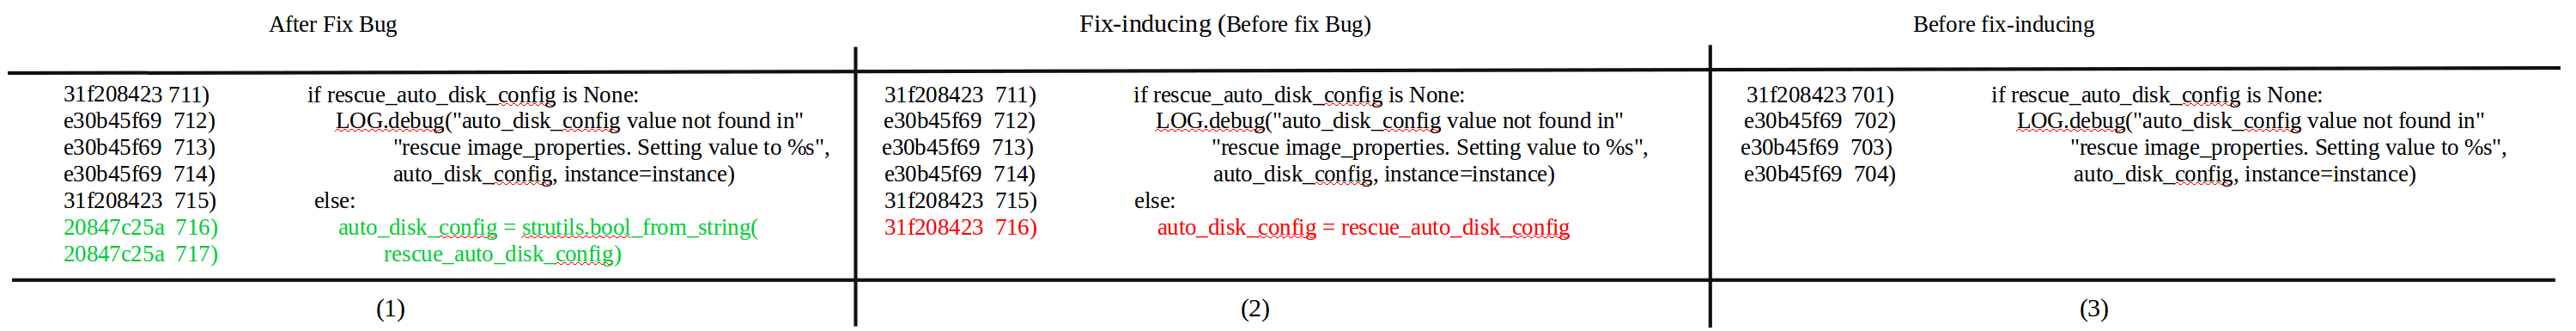
\includegraphics[height=2in, width=7in]{responsible.png}
\caption{Example of when the previous commit,31f208423, inserted the bug}
\label{fig:1}       % Give a unique label
\end{figure*}

\begin{figure}[htb]
\centering
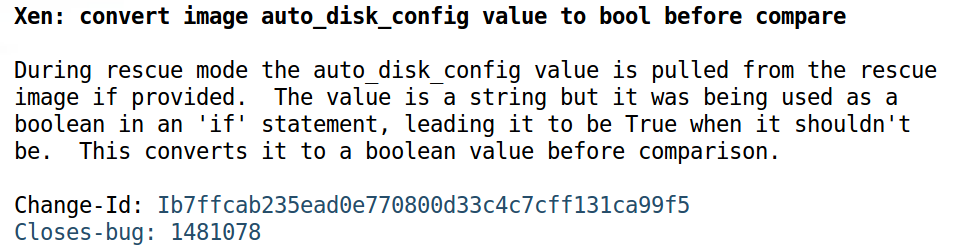
\includegraphics[height=2.4cm]{gerritPrevCommit.png}
\caption{Description of the bug-fix commit when the previous commit caused the bug}
\label{fig:2}       % Give a unique label
\end{figure}

\begin{figure*}[htb]
\centering
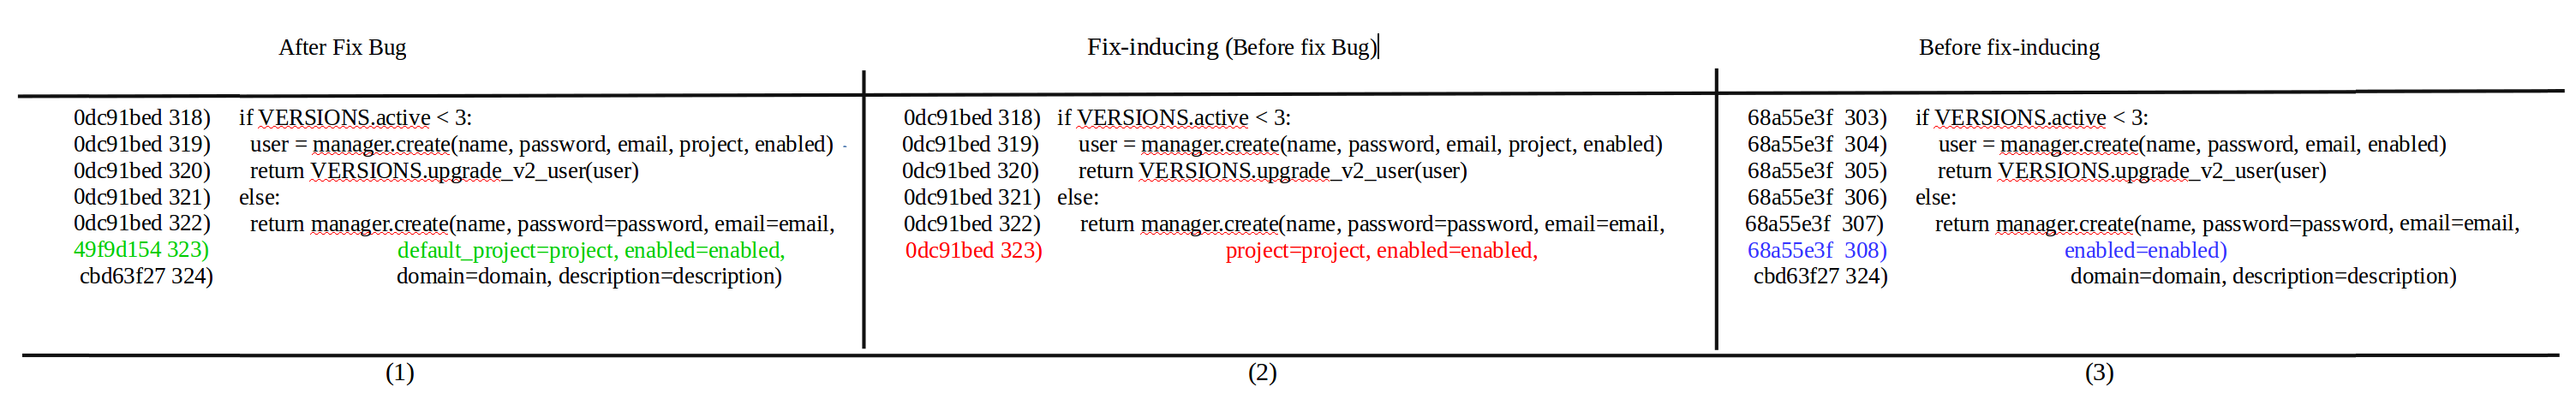
\includegraphics[height=2in, width=7in]{noResponsible.png}
\caption{Example of when the previous commit,0dc91bed, did not inserted the bug}
\label{fig:3}       % Give a unique label
\end{figure*}

\begin{figure}[htb]
\centering
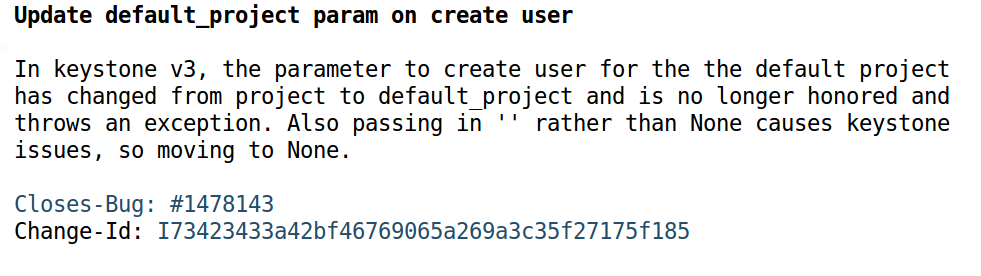
\includegraphics[height=2.4cm]{UpdateFixBug.png}
\caption{Description of the bug-fix commit when the previous commit dind't cause the bug}
\label{fig:4}       % Give a unique label
\end{figure}

The remainder of this paper is structured as follows. First, we present the motivations that support our study,  explaining the current body of knowleadge in section~\ref{sec:related}. Then, Section~\ref{sec:methodology} describes the methodology used to identify the moment in which the bug was inserted in the source code, followed by the results obtained after applaying our approach to OpenStack in Section~\ref{sec:results}. Section~\ref{sec:discussion} discusses potential applications and improvements of our approach. Section~\ref{sec:threats} reports threats to validity. Finally, Section~\ref{sec:conclusions} concludes the article.

\section{Related Work}
\label{sec:related}
The first algorithm to identifying bug-introducing code changes automatically was described in \cite{sliwerski2005changes}. Currently, is a well-known algorithm called SZZ, which is based on text diferencing to discover modified, added and delete lines between the bug-fix and its previous version. SZZ uses CVS annotate command to identify the last commit that touched these lines.

An improvement on SZZ algorithm is described in \cite{kim2006automatic}, the authors used annotation graphs instead of CVS annotation to locate, in previous versions, the affected lines by modification and deletion. Also, they deleting some false positives as blank spaces, changes in the format or changes in the comments.

Other methodology to identify the origins of a bug is describes in \cite{sinha2010buginnings}, this work doesn't present a text-based technique as SZZ, the authors analized the effects of bug-fix changes on program dependences. Taking into account the semantic of the source code they achieved more accuracy identifying the origins of a bug.

These two approach have the similar ideas: (1) find the differences between the bug-fix version of and the previous version of the file to recognize those changes done by bug-fix commit. (2) look back in the code revision history until identify which version touched the lines affected in the bug-fix for the last time.

Exists several articles based on SZZ such as \cite{williams2008szz} revisied SZZ algorithm, tracking bug-inducing changes and identify change types of them. Also, in \cite{yangbug} the authors applyed this algorithm to find out what kind of bug-inducing changes are likely to become in a great threat after being marked as bug-fix changes.In addition, new techniques in bug prediction are based in this algotimh such as \cite{kim2008classifying} which was the first work classifying file changes as buggy or clean using change information features and source code terms.

%In addition some tools are based on SZZ too such as \cite{} 
Finally our idea.

\section{Methodology}
\label{sec:methodology}
%We present our approach to identify how and where a bug was inserted into the source code, causing a later fix. 
We extract all the data necesary to analyze when the bug was inserted from the issue tracking system and the code review system used by the project we are analyzing. OpenStack uses Launchpad\footnote{\url{https://launchpad.net/openstack}} and Gerrit\footnote{\url{https://review.openstack.org/}}.

The Launchapd of each project works with issues reports called tickets, which describe bug reports, feature requests, maintenance tickets, and even design discussions. But, in our study we are only interested in those tickets that describe a bug report and, in addition, have been closed with a merged in the code source to fix the bug. In this bug reports we can find a comment with the link of Gerrit where the bug was fixed. Is in Gerrit where we can see all the patchsets proposed and the comments done by the reviewers. 

\subsection{Fist Stage: The Filtering}
\label{sec:firstStage}
In our approach, first of all we must identifying which of those issues extracted from Launchapd are bug reports. But, this is not a trivial task and we performed this identification using a web tool\footnote{\url{bugtracking.libresoft.es}} development to provide the researcher with all the relevant information needed to decide if an issue corresponds to a bug report or not. The tool uses information extracted automatically from the project repositories, and offers a web-based interface which allows for collaboration, traceability and transparency of the identification of bug reports.

During the identification of the issues we have to take into account the next parameters for each ticket, the title and the description of the issue report and the description of the fix commit. Also, the code changes if neither the descriptions and the comments clarified the underlying ticket. Each ticket was then categorized into one of three following groups.
\begin{enumerate}
  \item The ticket describes a bug report.
  \item The ticket describes a feature, an optimization code, changes in test files or other not bug reports.
  \item The ticket presents a vague description and cannot be classified without doubts.
\end{enumerate}

Henceforth, we will refer to Group 1 as \textit{Bug Report}, Group 2 as \textit{Not Bug Report} and Group 3 as \textit{Undecided}.

As result of analyze the tickets, main differences extracting data and to classifying tickets were found. So, we agree to follow the next four criteria: 
\begin{itemize}
    \item When there are only test files in the ticket, we classified it as note being a bug report. Test files in a ticket will not be analyzed, they are indispensables and used as testing method to determine whether the code is fit for use. Sometimes the developers inserted the bug only in the test files, in these cases the ticket was not considered as bug report because the software works as expected only failed the test.
    \item When the title described optimization, deletion of a dead code or the implementation of new characteristics, our criteria indicated that it was not a bug report because there is no failure. 
    \item When the title described the program as not working as expected, our criteria indicated that it was a bug report. 
    \item When the title described that updates were required, our criteria indicated that it was a bug report. We consider all tickets that require updating as bug reports, because updating a software hints to the software not operating as expected. 
\end{itemize}

Sometimes we were unable to answer all the questions due to having insufficient data or because of the complexity of the issue. In this case, the ticket was classified into the \textit{Undecided} group.
\subsection{Second Stage: Responsability of Previous Commit}
\label{sec:secondStage}
The next part is focusing on analyzing the previous commit in the \textit{Bug Report} group. For that, we had to analyze the lines involved in the bug fix, in the commit parent of the bug fix commit, and be sure that the lines was inserted/modified in the previous commit. This, way we can sure that the previous commit didn't copied any line that contained the bug, because in this case, the previous commit is not responsible to cause the bug. 

The analisys was done manually, and we used \textit{git blame} to see all the previos commit in each line of a involved file. Also, we used \textit{diff} to see all the differences between two files, in our case, the file is going to be the same but in different moment inside the control version system used.

Te procedure following in each file involved in a fix bug is describing below;
\begin{enumerate}
  \item git checkout \textit{commmit that fix the bug}, git blame \textit{file involved}. In this step we can see the lines added, modified or deleted by the commit that fix the bug.
  \item git checkout \textit{parent of commmit that fix the bug}, git blame \textit{file involved}. In this step we can see all the previous commits involved in the different lines touched in the fix bug.
  \item git checkout \textit{parent of previous commit}, git blame \textit{file involved}. In this step we can esure that the previous commit inserted these lines.
\end{enumerate}


Finally we need to discard some noise presents in our final resulst according to the responsability of the previous commit inserting the bug in the code source. Due to they were not responsibles for cause the bug, we delete those previous commit which presents the following criteria;
\begin{itemize}
    \item Blank lines
    \item Format changes
    \item Copied lines
    \item Changes in the comment.
    \item Updatings in the version of a file. 
\end{itemize}


\section{Evaluation}
\label{sec:evaluation}

We validate our methodology anlayzing 459 tickets in OpenStack. OpenStack was particularly of interest because of its continuously evolving due to its very active community. Although its short life, only five years, more than 5 thousand of resarchers and more than 233 thousand of commits with more than 2 Million of lines of code have contributed in the development of the project \footnote{\url{http://activity.openstack.org/dash/browser/}}. Futhermore, all history is saved and available in a version control system, being able to access to its issue tracking system \footnote{\url{https://launchpad.net/openstack}} and the source code review \footnote{\url{https://review.openstack.org/}}

OpenStack is composed by 9 projects, but we only focused in the four of them, Nova, Cinder, Neutron and Horizon as we can see in table \ref{tab:OpenStack} these projects are really actives during all their history and in the last year.
\begin{table}[htb]
\centering
%\begin{center} {\footnotesize
\caption{ Commits per Project in OpenStack}
\label{tab:OpenStack}
\begin{tabular}{lll}
\toprule[0.3mm]%{\smallskip}
  & All History \kern 1pc & Last Year (2015) \\\hline
Nova    \kern 1pc & 14,558 & 3,283 \\
Fuel    \kern 1pc & 9,139 & 5,123 \\
Netron  \kern 1pc & 8,452 & 3,855 \\
Horizon \kern 1pc & 4,871 & 1,994 \\
Cinder  \kern 1pc & 4,556 & 1,832 \\
Keystone\kern 1pc & 4,874 & 1,795  \\
Heat    \kern 1pc & 6,395 & 2,372  \\
Glance  \kern 1pc & 2,651 & 723 \\
Tempest \kern 1pc & 4,141 & 1,312 \\
\bottomrule[0.3mm]
\end{tabular} %}
%\end{center}
\end{table}

In this four projects we analized the relationship of bug fixes with their previous commits. In order to identify the moment in which the bug was injected into the source code. The first stage we did automatically using the tool and a double bind between three researchers, three PhD student  included me. The second stage was done manually and only me was involved analizing this relationship. %that, we extract a total of 459 tickets from this projects, in which we should be sure that the bug fixes come from a bug report, because two of five issues are misclassified \cite{herzig2013s} and this should cause bias in our final results.

\section{Results}
\label{sec:results}

We extracted a total of 459 different tickets from the Launchpad of the four principal projects in OpenStack, 125 tickets from Nova, 125 tickets from cinder, 125 tickets from Horizon and 84 tickets from Neutron. These tickets first, were analized to identify those ones which were real bug reports. And secondly, each file was analyzed to obtain which previous commit inserted the bug causing the failure of the system and reporting the bug report. 

\subsection{Fist Stage}
\label{sec:resultsFS}

We classify a total of 459 tickets using the tool. In 417 of the ticktes, we used double bind analysis, and only those tickets classified as bug report by two of us, were considered in the next stage to analyze the relevance of their previous commits.

The table \ref{tab:2} shows the percentage of each researcher after analyzing the tickets, and the number of tickets classifyed identically by two different researchers. Obtaining that the researchers R1 and R2 had a similar data in their results, whereas research R2 got results significantly differents with a higher number of tickets classifyed as Bug Report.
 
Finally, the researchers identifyed in the same way 292 tickets, that is, their results matched in a 70\% of the cases. Obtaining 209 tickets classifyed as Bug report, 74 tickets classifyed as Not Bug Report and 9 tickets classifyed as Undecided.

\begin{table}
\centering
%\begin{center} {\footnotesize
\caption{ Statistics of each researcher in the classification}
\label{tab:2}
\begin{tabular}{lllll}
\toprule[0.3mm]%{\smallskip}
  & Bug Report & Not Bug Report & Undecided & Total \\\hline
R1  & (184)55\% & (115)34\% & (35)11\% & 334 \\
R2  & (188)76\% & (54)22 \% & (7)3\% & 249 \\
R3 & (188)56\% & (116)35\% & (30)9\% & 334 \\
Finally & (209)72\% & (74)25\% & (9)3\% & 292 \\
\bottomrule[0.3mm]
\end{tabular} %}
%\end{center}
\end{table}

Also we had measured the concordance in the classification of each developer according to the project analized. The table \ref{tab:3} shows that the concordante got between all the three research was very similar, around a 70\%. Furthermore, the concordance form each researcher with the rest alwas was up to 60\%. 

\begin{table}[htb]
\begin{center} {\footnotesize
\caption{ Concordance between each developer in each repository}
\label{tab:3}
\begin{tabular}{llllll}
\toprule[0.3mm]%{\smallskip}
  & Nova & Cinder & Horizon & Neutron & Total\\\hline
R1\&R2   & (44)70\% & (40)77\%  & (37)60\% & -        & 68\% \\
R1\&R3   &  -        & (46)73\%  & (48)76\% & (26)62\% & 71 \% \\
R2\&R3   & (41)66\% & (10)100\% & -         & -        &  71\% \\
\bottomrule[0.3mm]
\end{tabular} }
\end{center}
\end{table}



\subsection{Second Stage}
\label{sec:resultsSS}

At this stage, we analyzed the 209 we got a list with all the previous commits and we were be able to classifyed the previous commit/s as Responsible, Not Responsible or Undecided, taken into account that the bug could be inserted in different lines of different commits, but not everyone had to be responsible for the commit, sometimes the previous commit copied lines from its previous commit or inserted comments and blank spaces. In fact, the responsible can be only one of them, more than one or maybe none.

We identifyed a total of 348 previous commits which can be responsible for inserting the line containing the bug. After analizing the Bug Reports and their previous commits and discarded 40 of them because were noise, Table \ref{tab:responsability}, we got that 152 previous commit were responsibles to cause the bug whereas 114 previous commit had not any responsability in the failure of the system, and only in 42 previous commits we were unable to identify the cause of the bug.

\begin{table}[htb]
\begin{center} {\footnotesize
\caption{ Responsability of each previous commit before and after deleting the noise in the results}
\label{tab:responsability}
\begin{tabular}{lcc}
\toprule[0.3mm]
  & \multicolumn{1}{c}{Before} & \multicolumn{1}{c}{After} \\
  & \multicolumn{1}{c}{Deleting Noise} & \multicolumn{1}{c}{Deleting Noise} \\\hline
\raisebox{1ex}{Responsible} & 152 & 152 \\[0ex]
\raisebox{1ex}{Not responsible} & 154 & 114 \\[0ex]
\raisebox{1ex}{Undecided} & 42 & 42 \\[0ex]
\bottomrule[0.3mm]
\end{tabular} }
\end{center}
\end{table}

Futhermore, focusing on how many previous commits presented each Bug Report, we obtained that 131 had one previous commit implicated, whereas 58 had more than one previous commit implicated in their file/s. According to Table \ref{tab:secondStage}, from the 131, we obtained that 65 of them inserted the bug, but 30 of them were not responsibles in the failure of the system. And from the 58 which had more than one previous commits, we obtained in total 189 previous commit, where 86 of them were respnsibles and 82 were not responsibles. %Probably, the bug was inserted in different lines of different commits, but not everyone has to be responsible for the commit, sometimes the previous commit copied lines from its previous commit or inserted comments and blank spaces. After the analysis the responsible can be only one of them, more than one or maybe none. 

\begin{table}[htb]
\begin{center} {\footnotesize
\caption{ Probability of cause the bug depending on how many previous commits had the bug report}
\label{tab:secondStage}
\begin{tabular}{lcc}
\toprule[0.3mm]
  & \multicolumn{1}{c}{One previous } & \multicolumn{1}{c}{More than one previous} \\
  & \multicolumn{1}{c}{commit} & \multicolumn{1}{c}{commit} \\\hline
\raisebox{1ex}{Responsible}     & 65 & 86 \\[0ex]
\raisebox{1ex}{Not responsible} & 30 & 82 \\[0ex]
\raisebox{1ex}{Undecided}       & 36 & 11 \\[0ex]
\bottomrule[0.3mm]
\end{tabular} }
\end{center}
\end{table}

Also, we looked the distribution of the previous commit in each Bug Report, Table \ref{tab:secondStage2}, we observed that the most commun distribuion in the relationship between previous commit and bug report is one previous commit per Bug Report, following by the second commun distribution, two previous commit per Bug Report.
\begin{table*}[htb]
\begin{center} {\footnotesize
\caption{ Distribution of number of previous commit per Bug Report in each project}
\label{tab:secondStage2}
\begin{tabular}{lccccc}
\toprule[0.3mm]
  & \multicolumn{1}{c}{One previous} & \multicolumn{1}{c}{two previous} & \multicolumn{1}{c}{three previous} & \multicolumn{1}{c}{four previous} & \multicolumn{1}{c}{+five previous}\\
  & \multicolumn{1}{c}{commit} & \multicolumn{1}{c}{commit} & \multicolumn{1}{c}{commit}& \multicolumn{1}{c}{commit}& \multicolumn{1}{c}{commit}\\\hline
\raisebox{1ex}{Neutron} & 11 & 3 & 2 & 2 & 0 \\[0ex]
\raisebox{1ex}{Horizon} & 39 & 8 & 3 & 2 & 4 \\[0ex]
\raisebox{1ex}{Nova} & 44 & 5 & 2 & 4 & 4 \\[0ex]
\raisebox{1ex}{Cinder} & 37 & 9 & 6 & 2 & 2\\[0ex]
\raisebox{1ex}{Total} & 131 & 25 & 13 & 10 & 10\\[0ex]
\bottomrule[0.3mm]
\end{tabular} }
\end{center}
\end{table*}

Finally we wanted to know the responsability preactised by each previous commit in the failure of a system, in other words, we were interested in analize from those cases where exists more than one previous commit, how many of them inserted the bug in the code source, Table \ref{tab:secondStage3}. We obtained that in 8 Bug Reports all the previous commits were responsibles, in 30 Bug reports at least one of their previous commit caused the bug and in 11 bug report none of their previous commits inserted the bug.
\begin{table*}[htb]
\begin{center} {\footnotesize
\caption{ Probability of cause the bug depending on how many previous commits had the bug report}
\label{tab:secondStage3}
\begin{tabular}{lccccc}
\toprule[0.3mm]
   & \multicolumn{1}{c}{two previous} & \multicolumn{1}{c}{three previous} & \multicolumn{1}{c}{four previous} & \multicolumn{1}{c}{+five previous} & \multicolumn{1}{c}{Total}\\
  & \multicolumn{1}{c}{commit} & \multicolumn{1}{c}{commit}& \multicolumn{1}{c}{commit}& \multicolumn{1}{c}{commit}\\\hline
\raisebox{1ex}{All Responsible}          & 4 & 3 & 0 & 1 & 8\\[0ex]
\raisebox{1ex}{At least one responsible} & 9 & 7 & 5 & 9 & 30\\[0ex]
\raisebox{1ex}{None Responsible}         & 4 & 2 & 4 & 1 & 11\\[0ex]
\raisebox{1ex}{Undecided}                & 1 & 0 & 1 & 0 & 2\\[0ex]
\bottomrule[0.3mm]
\end{tabular} }
\end{center}
\end{table*}


\section{Discussion}
\label{sec:discussion}
\fbox{\begin{minipage}{25em}
\textbf{RQ1:} asdasdasdasdasdasdsaddasdadasdasd
\end{minipage}}
\fbox{\begin{minipage}{25em}
\textbf{RQ2:} asdasdasdasdasdasdsaddasdadasdasd
\end{minipage}}
- Como se responden las RQ1 y RQ2
- No todos los casos son tan claros como los mostrados en los ejemplos ....
- Casuistica del common juidment
- Hemos sido conservadores
-Hemos utilizado la herramienta porque es un proceso complicado
Once we have all the tickets analyzed by diferents researchers who have used a double blind, how to proceed if there are discordances between them:
\begin{enumerate}
\item Should they discuss after their analysis to reach a better classification?, Should the tool provide this?
\item Does the Bug report only the same ticket classified as Bug report for all the researchers?
\end{enumerate}

How to proceed if looking for the responsability of a bug when only added lines are inserted? And we are talking about a bug report not a new feature, these kinds of cases use to be when a researcher forgot check some case inside a function. [reference]
\begin{enumerate}
\item Is responsible the function where these lines are content?
\item Is responsible the last commit that modify something in the function?
\end{enumerate}


\section{Threats to validity}
\label{sec:threats}
%The limited sample size of tickets used in this research is the major threat to its validity. %It may happen, that only with 100 seemingly random tickets, there may be a prior unknown tendency. This is in fact similar to~\cite{sliwerski2005changes}, where the trend indicates that most bugs are fixed on Fridays.
The size of the tickets extracted form the Launcpad is medium, but doing the analisys manually we are sure that the results present in this paper are valid, being sure that the previous commits classifyed as not responsible, they are. 

Although, we understand that the model presented has some threats, external and internal, that make our model not 100\% valid. The internal threats related to the researchers that have conducted the study are following:

\begin{itemize}
    \item We have not taken into account errors that have been classified into \textit{Undecided}, and probably we are lost some real bug reports belonging this group .
    \item There could be some lax criteria involving the subjective opinion of the researchers.
    \item The researchers are not experts in OpenStack, and our inexperience may have influenced the results of the analysis.
    \item We are only using part of the information that the ticket provides, like comments and text. There could be a recognized pattern in teh data, unknown at first sight, that involves other parts of the information.
    \item Although we use a random script to extract the tickets reported in during the last year, 2015, from the launchpad, in this year could be some bias unidentified.
    \item In case of the researchers didn't find the information to know if the previous commit inserted the bug or in contrast, it was caused by the evolution of the software. They keep the traditionalist thought, classify these previous commits are responsibles.
\end{itemize}

The external threats, related to the case of the project, are following:

\begin{itemize}
    \item The word \textit{bug} is continuously mentioned in the description and commit of a ticket even when we found it is not an error. This could lead to the incorrect classification during the reviewing process.
    \item Some tickets are not explicitly described, which could increase the percentage of \textit{Undecided}. This is especially true if the reviewers are not from OpenStack.
    \item OpenStack is a special project put down a constant evolution due to their active community of developers. Maybe, in other projects with less commits per year the statistics about the responsability of previous commit change.
\end{itemize}


\section{Conclusions and Future Work}
\label{sec:conclusions}
The empirical experiment carried out in OpenStack, supported that the current premisse assumed does not hold for a large fraction of the analyzed bugs, because around the 40\% of the previous commits were not responsibles inserting the bug.
With our results we can identify which ones are real changes that introduced the bug, and this could be useful to improve the accuracy of those tools developed to prevent bugs. Also, the software developers stand to benefit from identifying where the bug was inserted, improve their methodology.
%How to plan to apply the knowledge in a way that can benefit software engineers.
%What are the anticipated contributions of the work?  How will you evaluate them to demonstrate usefulness?

A final field in our future work concerns the full automatization on the methodology could developer an automatic classifier base on the idea that not all the previous commit injected the bug. Another interesting investigation could leadge the same empirical study in a project with a community less active, to can prove if our idea is fullfil in other projects.

%ACKNOWLEDGMENTS are optional
\section{Acknowledgments}
We thank the two phd students, Dorealda Dalipaj and Nelson Sekitoleko, that participated differentiating Bug report from the others. Also, we thank Bitergia \footnote{\url{http://bitergia.com/}} to explain its available database of OpenStack. 
Finally,thanks the Spanish Goverment because all authors are funded in part by it, through project TIN2014-59400-R.

\nocite{*}
%
% The following two commands are all you need in the
% initial runs of your .tex file to
% produce the bibliography for the citations in your paper.
\bibliographystyle{abbrv}
\bibliography{sigproc}  % sigproc.bib is the name of the Bibliography in this case
% You must have a proper ".bib" file
%  and remember to run:
% latex bibtex latex latex
% to resolve all references
%
% ACM needs 'a single self-contained file'!
%
%APPENDICES are optional
%\balancecolumns
\end{document}
